
\section{\texorpdfstring{\MakeUppercase{exploring active galactic nuclei with gravitational waves}}{exploring active galactic nuclei with gravitational waves}}
\label{sec:chapter-agnbbh}

\counterwithin{figure}{section}
\counterwithin{table}{section}

\par The model and results described in this chapter were published in the \textit{Astrophysical Journal} \citep{McKernan+25-mcfactsI}.
As such, the main text of this chapter is directly informed by the content of our publication.
To cite this chapter, please use \citet{McKernan+25-mcfactsI}.

\subsection{Motivation}

AGN are a promising source of the BBH mergers observed in gravitational waves with LVK.
Constraining the AGN channel allows us to limit AGN parameter space (disk density, size, average lifetime) and NSC parameter space.
Constraints on AGN and NSCs have implications for $\Lambda$CDM models of AGN feedback and models of AGN-driven SMBH merger and growth.
Here we present several qualitative studies of the AGN channel using a public, open-source, fast, reproducible code \code{McFACTS}\footnote{https://github.com/mcfacts/mcfacts}:Monte Carlo for AGN channel Testing \& Simulation.
We demonstrate several important features for testing the AGN channel, including:
i) growth to large mass IMBH is helped by the presence of migration traps or swamps,
ii) flat BH initial mass functions highlight hierarchical merger features in the mass spectrum,
iii) the $q$--$\Xeff$ anti-correlation is a strong test of the bias to prograde mergers in the AGN channel,
iv) spheroid encounters can drive a fraction of mergers with high in-plane spin components ($\chi_{\rm p}$),
v) a high rate of EMRIs are driven by an initial population of embedded retrograde BH, and
vi) both LVK and LISA are powerful probes of models of AGN disks and their embedded populations.


\subsection{Default Model Assumptions}
\label{sec:mcfacts-assumptions}

In the results that follow, default model parameters (also in \code{p1_model_default.ini}) are listed in Table~\ref{tab:default_model}. Unless otherwise specified, we assume a \citet[][hereafter SG]{SirkoGoodman03} disk model as interpolated from the \code{pAGN} package \citep{Gangardt+24-pAGN} around a $10^{8}\,M_{\odot}$ SMBH, spanning $[6,50000]\,\Rg$, with disk viscosity parameter $\alpha=0.01$ and lasting $0.5$ Myr. Average disk aspect ratio for this model is assumed to be $\sim 0.03$ and EMRIs are tracked within $50\,\Rg$ of the SMBH. A migration trap is assumed to live at $700\,\Rg$ (\citealt{Bellovary+16}, although see also \citealt{Grishin+23}). 

Following \citet{Generozov+18}, a NSC is assumed to fill the inner galactic nucleus out to $5$pc, with an inner number density profile $n\propto r^{-7/4}$ within $r\sim 0.25$pc and $n \propto r^{-2.5}$ outside that. The BH population of the NSC is normalized at $10^{4}$ inside the central ${\rm pc}^{3}$, matching inferences of the population in our own Galactic nucleus. The BH population mass distribution has a Pareto form with index $M^{-2}$, $M_{\rm BH, min}=10\,M_{\odot}$, $M_{\rm BH,max}=40\,M_{\odot}$. BH drawn from this distribution above $M_{\rm BH,max}$ are randomly assigned masses in a Gaussian pile-up centered on $35\,M_{\odot}$ of width $2.3\,M_{\odot}$, mimicking the observed pile-up in the LVK mass spectrum \citep{Abbott+23-massbump}. The initial BH spin distribution is assumed to be drawn from a Gaussian centered on dimensionless spin parameter $=0$ and of width $0.1$. Assuming an average scale height across the \citet{SirkoGoodman03} disk model, the fraction of BH with orbits coincident with the disk volume is calculated and the corresponding radial BH locations are generated from a distribution reflecting the user choice of NSC density.


Our default accretion rate assumptions for determining the change in mass, spin magnitude, and spin angle of each embedded black hole is that they accrete at Eddington, and must accrete $0.01$ of their own mass (while on a circular, prograde orbit) in order to have their spin aligned with the disk orbital angular momentum.
 
Our default assumption is a uniform distribution of eccentricity, i.e. sub-thermal, allowing for e.g. only partial recovery from a previous AGN episode that might have dynamically cooled these orbits. The uniform distribution is capped at some initial eccentricity value $e_{\rm max}$ to test the likely rate of relaxation from a previous AGN episode.
A full range of initial eccentricity distributions is tested in \citet{Cook+25} (presented in the next chapter).

 We assume that gas hardening of BBH follows the prescription in \citet{Baruteau11}. Our default model allows for dynamical interaction between the circularized population of BH in the AGN disk and the eccentric population (i.e. dynamics flag is on). 

Finally, we estimate the approximate merger rate corresponding to a particular simulation, by assuming a number density of AGN $n_{\rm AGN} \sim 10^{-3} \,{\rm Mpc^{-3}} \sim 10^{6} \,{\rm Gpc^{-3}}$. This yields the very useful approximation~\footnote{ Dong Lai, private communication} that $\mathcal{R}=1$ merger/AGN/Myr in these simulations is equivalent to a rate of $\mathcal{R}=1\,{\rm Gpc^{-3} yr^{-1}}$. We caution this is only an approximate rate estimate, as we are not accounting for the variation in merger rates or the distribution of merger parameters that may occur with variations in SMBH mass, NSC mass and AGN disk model. Such complications are explored in \citet{Delfavero+25-mcfactsIII}, where we attempt to simulate the AGN channel for the universe, with a distribution of galaxy properties.

\subsection{Testing Models with McFACTS}
\label{sec:mcfacts-testing}

\subsection{Testing nuclear star cluster models}
Using the default values outlined above, Fig.~\ref{fig:mf2} (left panel) shows the number of BBH mergers as a function of remnant mass.
In Fig.~\ref{fig:mf2} (left panel), the mass function of merged BH peaks between $[20,30]\,M_{\odot}$, with a secondary peak at $\sim [40,50]\,M_{\odot}$. The dominant, lower-mass peak is driven by mergers among the most numerous low mass BH in the initial mass function (IMF, $\sim [10,15]M_{\odot}+[10,15]\,M_{\odot}$). The second peak is driven by mergers between masses in the pile-up and the low masses ($\sim [35]\,M_{\odot} + [10-15]\,M_{\odot}$), since the former are the fastest migrators and the latter are the most common BH. The equivalent mean merger rate is $\mathcal{R}\sim 22.0\,{\rm Gpc}^{-3}{\rm yr}^{-1}$.

By contrast, Fig.~\ref{fig:mf2} (right panel) shows the same quantities, for the same BH minimum and maximum mass and toy-model pile-up but with $M_{\rm BH} \propto M^{-1}$. Qualitatively we can see that a flatter IMF drives more numerous and more massive mergers typically, with a longer tail to high mass and a significant number of IMBH ($>100\,M_{\odot}$) produced. The equivalent mean merger rate is $\mathcal{R}\sim 40.0\,{\rm Gpc}^{-3}{\rm yr}^{-1}$. Here, a flatter IMF reverses the magnitudes of the two peaks in Fig.~\ref{fig:mf2} (left panel), with the peak between $\sim [45,55]\,M_{\odot}$ dominating the merger spectrum. We also observe the emergence of a third peak at $\sim [65,75]\,M_{\odot}$, followed by a long hierarchical tail to higher masses. The toy model pile-up between $[35,40]\,M_{\odot}$ is relatively more prominent for a $M^{-1}$ IMF so both this feature and mergers among BH in this feature (at $[70,75]\,M_{\odot}$) are significantly more prominent than in the left panel. The new, third peak is an echo of the pile-up in the IMF yielding BH around $\sim 70\,M_{\odot}$ due to $\sim 35\,M_{\odot}+35\,M_{\odot}$ mergers since the relatively numerous massive BHs ($\sim 35\,M_{\odot}$) migrate fastest and tend to find each other more quickly. This picture is confirmed in Fig.~\ref{fig:m1m2} where we see an excess merger rate among the 1g-1g (gold) population in the right panel at $30-40$ in $M_{1}$ and indeed at ($M_{1},M_{2}$)$\sim 30-40\,M_{\odot}$ compared to the left panel. Intriguingly, there may be hints of an echo of the $35\,M_{\odot}$ peak in LVK's third observing run (O3) data at $\sim 70\,M_{\odot}$ which, if true, are suggestive of hierarchical mass mergers in a deep potential well \citep{Ignacio24}.  Observations of a relatively faint echo feature around $\sim 70\,M_{\odot}$ implies an IMF $\propto M^{[-1.5,-2]}$ for the AGN channel, but also requires a lower fraction of low mass BH to minimize intermediate features. Possibly a broken powerlaw IMF may be required as an input to AGN channel models. Or kicks may be important in segregation of generations between short-lived AGN phases. The relative positions and strengths of such peaks may be key in disentangling different BBH formation pathways in LVK data. For example, if in O4-O5, higher mass peaks are observed among $70M_{\odot}+70_{\odot}$ and $140_{\odot}+70_{\odot}$ BBH, these would be extremely suggestive of mergers retained in a very deep potential well, since such high generation and high spin mergers are very unlikely to be retained in clusters \citep[see also][]{FordMcKernan25}. The magnitude and relative sizes of such echo features in the mass spectrum will be explored more thoroughly in future work. 

\begin{figure*}
    \centering
    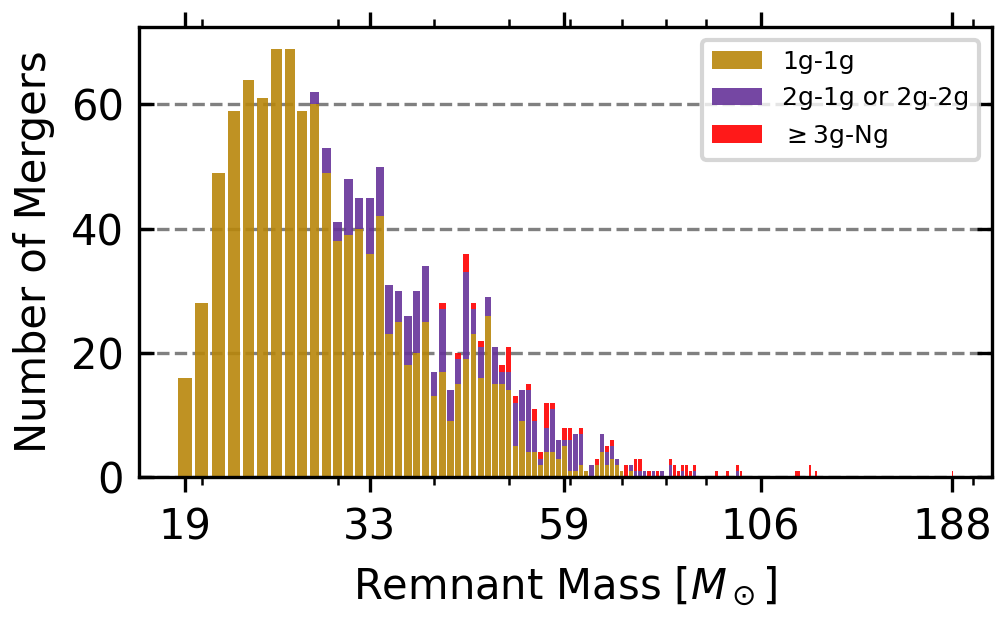
\includegraphics[width=0.5\textwidth]{ch_agnbbh_figs/default_merger_remnant_mass.png}
      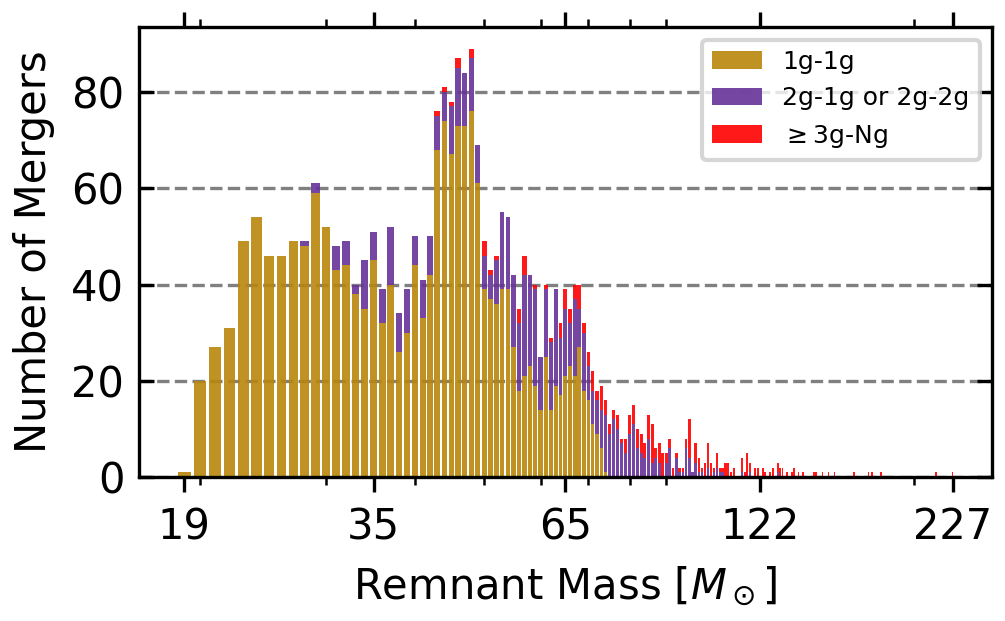
\includegraphics[width=0.5\textwidth]{ch_agnbbh_figs/p123_m1_merger_remnant_mass.png}
	\caption[Number of BBH mergers per generation of BH as a function of merged mass]{\textbf{Number of BBH mergers per generation of BH as a function of merged mass} ($M_\odot$) for different BH initial mass functions (IMFs). Left panel corresponds to a BH IMF of $M^{-2}$ with minimum $M_{\rm BH}=10\,M_{\odot}$, maximum initial mass $M_{\rm BH, max}=40\,M_{\odot}$ and simple pile-up model between $[35,40]\,M_{\odot}$ for a 0.5Myr, \citet{SirkoGoodman03} disk model around a $M_{\rm SMBH}=10^{8}\,M_{\odot}$ (see text). Gold denotes 1g-1g mergers, purple denotes 2g-mg ($m\leq 2$)and red denotes 3g-ng ($n \leq 3$) and higher, where 1g is first generation BH (not previously involved in a merger), 2g is second generation (the result of 1 merger) etc. Right panel is as left panel but with BH IMF of $M^{-1}$. Input file is \texttt{model\_choice\_old.ini} with \texttt{nsc\_imf\_bh\_powerlaw\_index = 2.(1.)} left (right), \texttt{galaxy\_num = 100} and \code{seed = 3456789018}. Equivalent merger rates correspond to $\mathcal{R}\sim 22.0(40.0) \,{\rm Gpc}^{-3} \rm {yr}^{-1}$ in left (right) panelin .
   }
    \label{fig:mf2}
\end{figure*}

\begin{figure*}
    \centering
    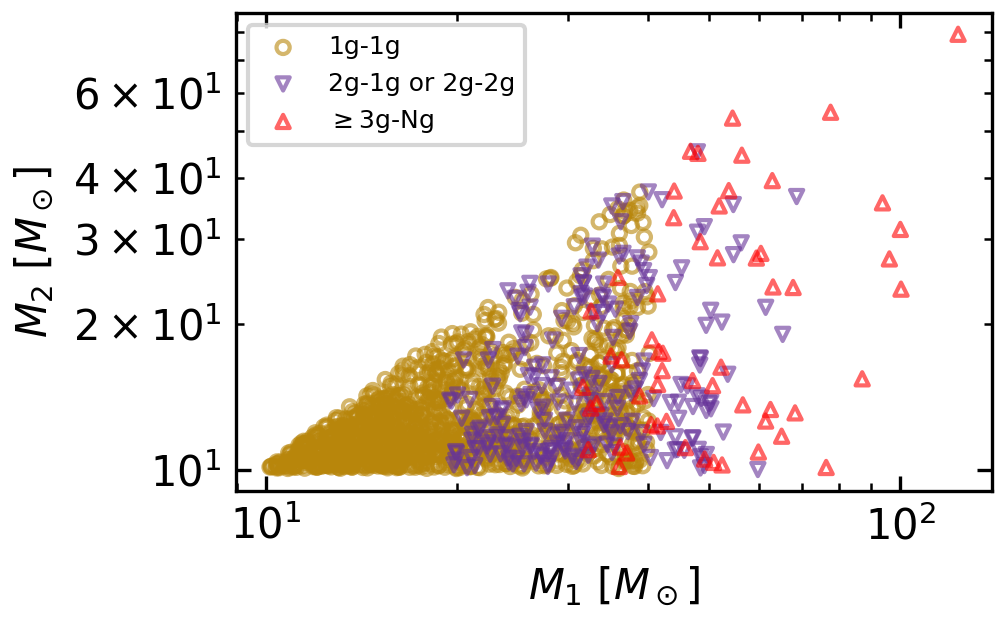
\includegraphics[width=0.5\textwidth]{ch_agnbbh_figs/default_m1m2.png}
      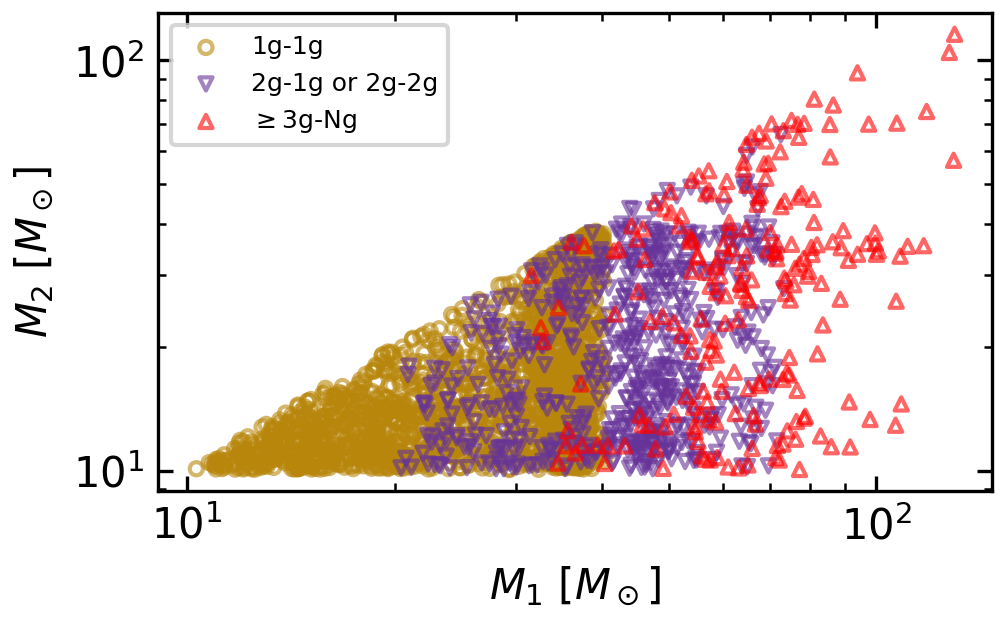
\includegraphics[width=0.5\textwidth]{ch_agnbbh_figs/p123_m1_m1m2.png}
	\caption[Distribution of merger BH masses]{Distribution of BH masses ($M_{1},M_{2}$) involved in the mergers in Fig.~\ref{fig:mf2}.
   }
    \label{fig:m1m2}
\end{figure*}

\subsection{The effect of orbital eccentricity damping}
AGN disks damp the orbital eccentricity of prograde orbiters over time \citep[e.g.][]{McKernan+12} but if the surface density increases with radius (as is the case in the inner region of the \citet{SirkoGoodman03} disk model) orbital eccentricities of retrograde orbits can be pumped \citep{Secunda+21}.

Since $t_{\rm damp} \propto h^{4}$, orbital eccentricity damping is fastest in thin parts of disk models ( e.g. $\sim [10^{2},10^{4}]\,\Rg$ in \citealt{SirkoGoodman03}). Therefore we expect BH orbits to circularize fastest in the thinnest parts of the disk. Since BBH formation is predominantly drawn from the population that have already circularized, we expect the BBH population to tend to form in the thinner parts of the disk model first.
 
If we assume an initially thermal distribution of orbital eccentricities, we expect an orbital distribution function 
\begin{equation}
    f(e){de} = 2e \;{de}
\end{equation}
such that the median orbital eccentricity is $e \sim 1/\sqrt{2} \sim 0.7$ and there is a uniform probability distribution of $e^{2}$. For initially thermal eccentricity distributions, we draw from a uniform distribution [0,1] to obtain $e^{2}$ at $t=0$. However, such a distribution is the limiting case where orbits have had sufficient time to relax and will only apply where there is a very long interval between AGN episodes. Instead, for our default case, which involves a short (0.5Myr) AGN lifetime, we introduce a maximum initial eccentricity ($e_{\rm max}$), capping the uniform distribution, corresponding to a relatively short period of relaxation between AGN episodes.

We expect new BBH to form mostly from the circularized population. The subsequent migration of such BBH either inwards or outwards, away from this disk region, will make dynamical encounters with eccentric orbiters more likely. Such encounters will be capable of either hardening, softening/ionizing the BBH, depending on the details of the encounter \citep[e.g.][]{Leigh+18,WangZhuLin24}. Note also $a \sim 10^{3}\,\Rg$ is a plausible location for a migration trap \citep{Bellovary+16} in such a disk, although \citet{Grishin+23} suggest that such traps can occur at radii $\times 3-5$ further out in the disk.

\begin{figure*}
    \centering
    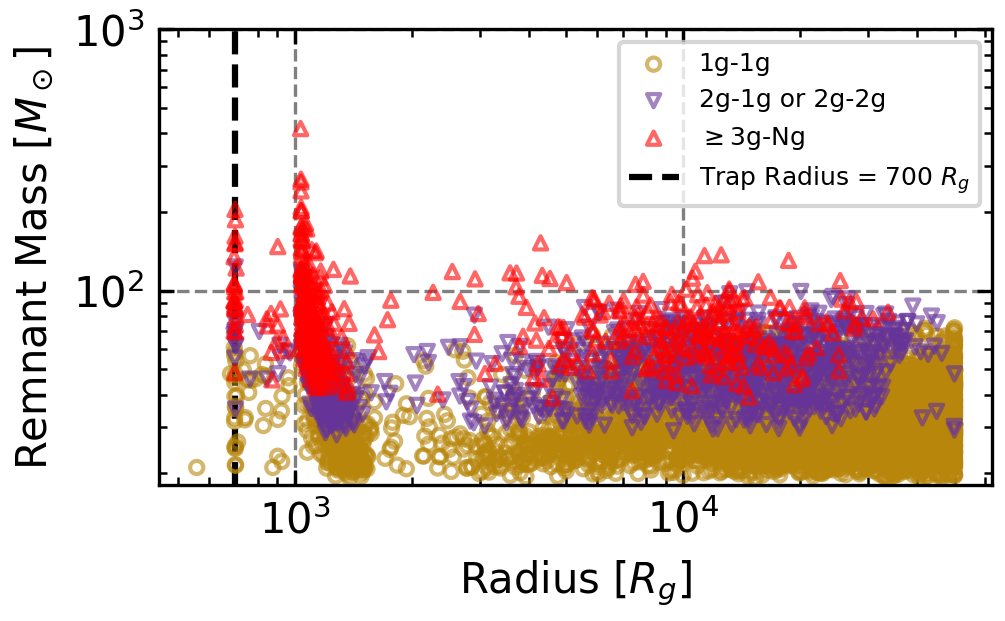
\includegraphics[width=0.5\textwidth]{ch_agnbbh_figs/p123_circ_merger_mass_v_radius.png}
      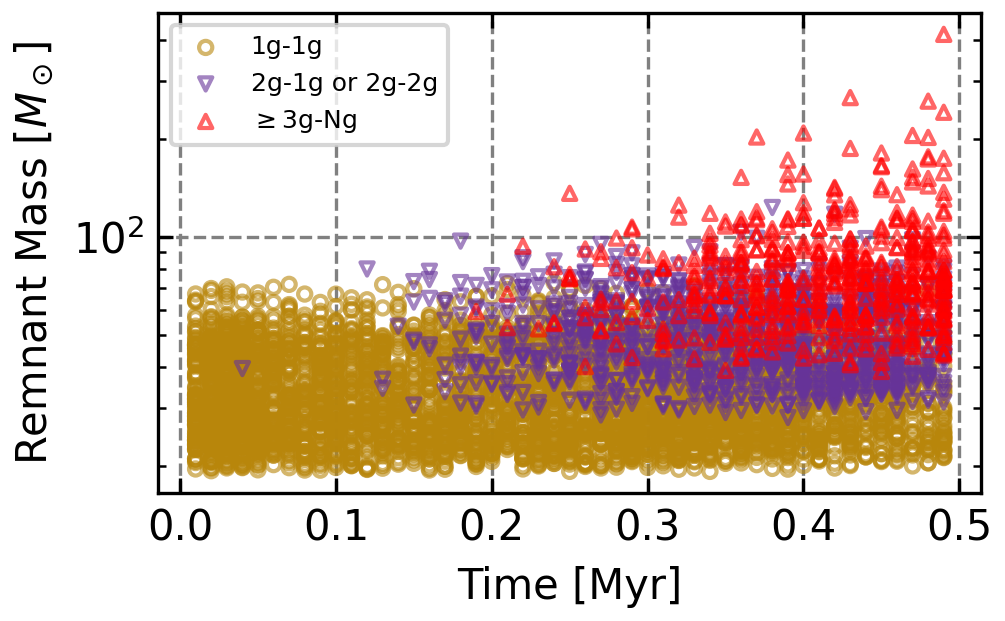
\includegraphics[width=0.5\textwidth]{ch_agnbbh_figs/p123_circ_time_of_merger.png}
	\caption[BBH merger mass as a function of disk radius and time]{\textbf{BBH merger mass as a function of disk radius (left panel) and time (right panel).} All BH are assumed initially circularized and no dynamical encounters occur. Input file is \texttt{model\_choice\_old.ini} with \texttt{flag\_orb\_ecc\_damping = 0}, \texttt{flag\_dynamic\_enc = 0}, \texttt{nsc\_spheroid\_normalization = 0.0}, \texttt{galaxy\_num = 100} and \texttt{seed = 3456789018}. Equivalent merger rate is ${\mathcal{R}} \sim 95.4\, {\rm Gpc}^{-3} {\rm yr}^{-1}.$
   }
    \label{fig:circ}
\end{figure*}





Fig.~\ref{fig:circ} shows the BBH merger masses as a function of disk radius (left panel) and time (right panel) for the setup as in Fig.~\ref{fig:mf2}, except all the BH are assumed to be initially circularized and we do not allow dynamical interactions. Feedback is on, so migration develops an outward component in the outer disk (driving a small pile-up near the outer disk edge). The equivalent merger rate is very high $\mathcal{R} \sim 95.4\,{\rm Gpc}^{-3} {\rm yr}^{-1}$ as BBH mergers start straightaway ($t=0$, right panel) and high generation mergers (2g,3g) quickly appear in $<0.1$ Myr. There is a divergence in the mass distribution of mergers in the right panel with IMBH-building mergers ($>100M_{\odot}$) starting in the first $\sim 0.2$ Myr, and growing larger over time. These  IMBH mergers occur preferentially at both the migration trap \citep{Bellovary+16}, and the migration swamp in front of the trap around $\sim 10^{3}\Rg$, where the Paardekooper migration torque drops by $\sim 30\%$ for $M_{\rm SMBH} \sim 10^{8}M_{\odot}$, leading to a pile-up at this region (see e.g. Fig.2 in \citep{Grishin+23} for an approximate illustration). The bulk of mergers are at lower mass, which was also the pattern we found in \citet{McKernan+20a} where we assumed all the BH are on circularized orbits at $t=0$. 

The largest mass IMBH occur at or near the migration trap or at the disk outer boundary. Some IMBH-producing mergers (up to $\sim 150\,M_{\odot}$) occur far from the trap, in regions of the disk where the size of the BBH Hill sphere radius is large. 

\begin{figure*}
    \centering
    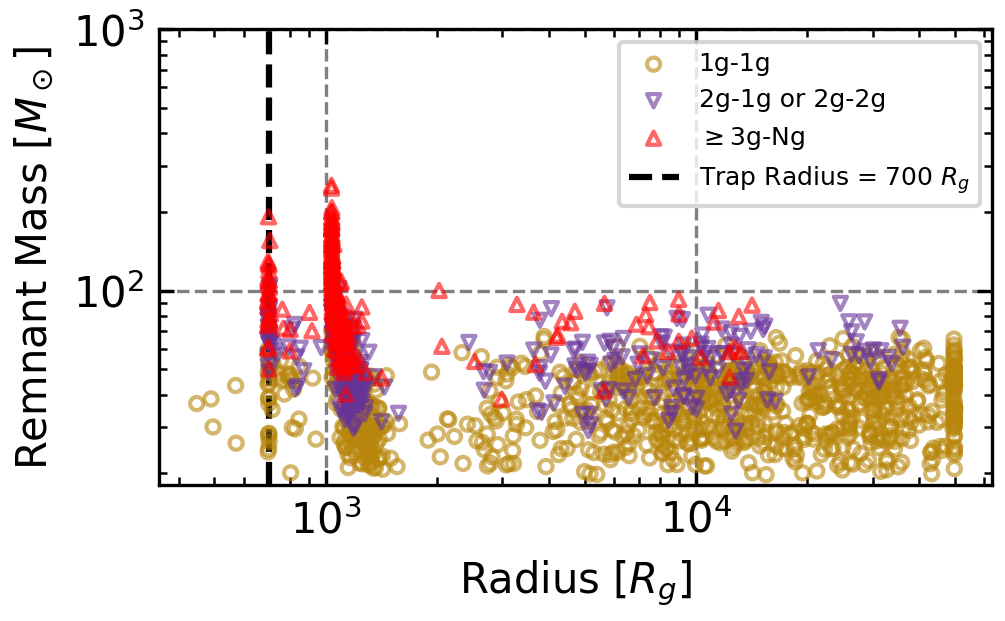
\includegraphics[width=0.5\textwidth]{ch_agnbbh_figs/p123_ec9_merger_mass_v_radius.png}
      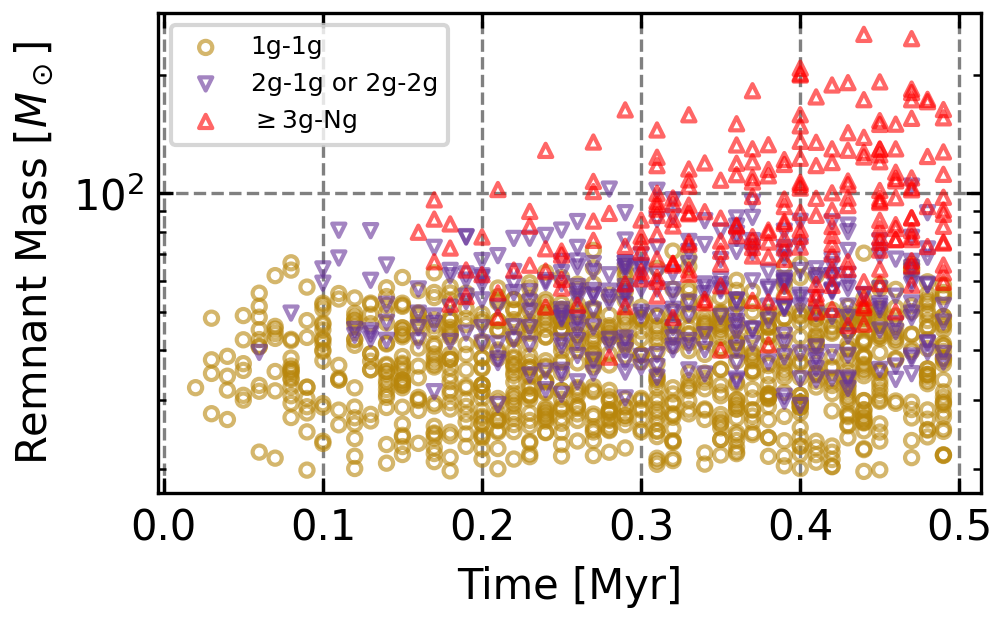
\includegraphics[width=0.5\textwidth]{ch_agnbbh_figs/p123_ec9_time_of_merger.png}
	\caption[BBH merger mass for e=[0.0,0.9]]{\textbf{BBH merger mass for e=[0.0,0.9]}As Fig.~\ref{fig:circ} except all BH are assumed to be drawn from an initial uniform distribution of orbital eccentricities between [$0.0,0.9$] and no dynamical encounters occur. Input file is as Fig.~\ref{fig:circ}, except \texttt{flag\_orb\_ecc\_damping = 1} and \texttt{disk\_bh\_orb\_ecc\_max\_init = 0.9}. Equivalent merger rate is ${\mathcal{R}} \sim 26.8 \,{\rm Gpc}^{-3} {\rm yr}^{-1}.$
   }
    \label{fig:ecc}
\end{figure*}

\begin{figure*}
    \centering
    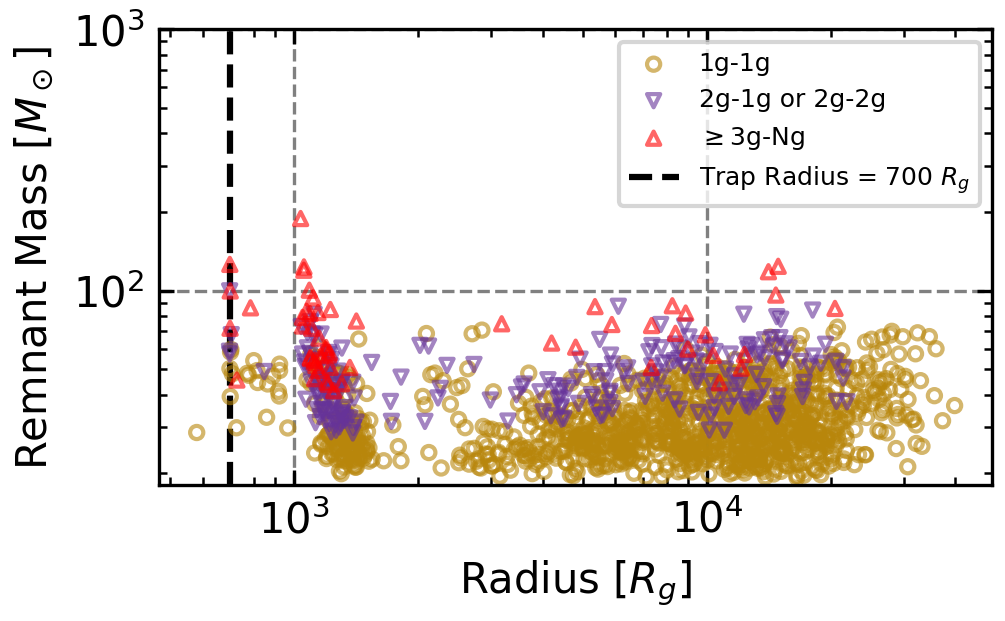
\includegraphics[width=0.5\textwidth]{ch_agnbbh_figs/default_merger_mass_v_radius.png}
      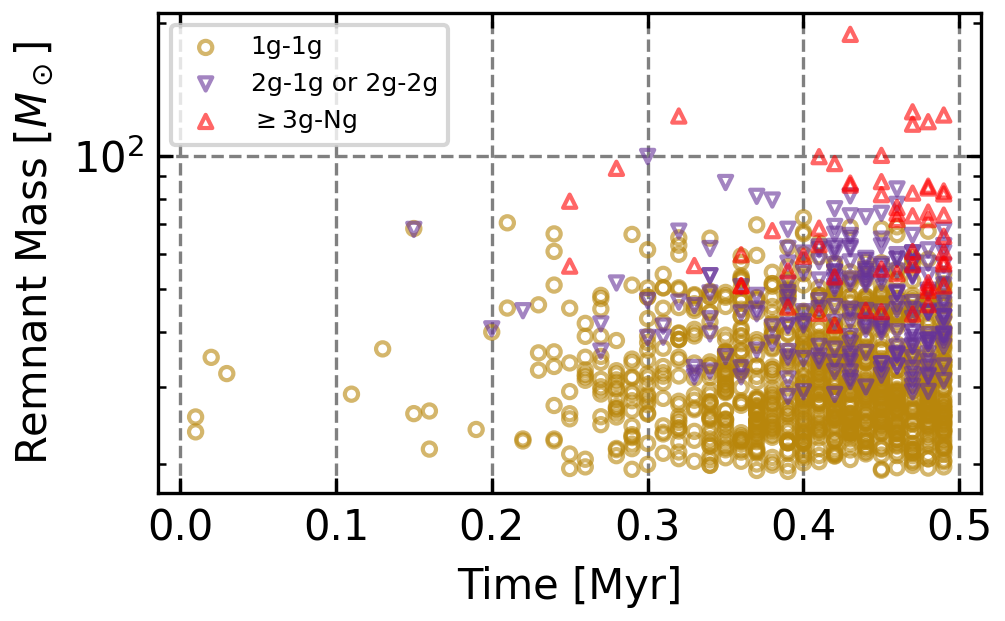
\includegraphics[width=0.5\textwidth]{ch_agnbbh_figs/default_time_of_merger.png}
	\caption[BBH merger mass for e=[0.0,0.3]]{\textbf{BBH merger mass for e=[0.0,0.3]}As Fig.~\ref{fig:ecc} except all BH are assumed to be drawn from an initial uniform distribution of orbital eccentricities between [$0.0,0.3$] and dynamical encounters are allowed. Input file is \texttt{model\_choice\_old.ini} with \texttt{flag\_orb\_ecc\_damping = 1}, \texttt{flag\_dynamic\_enc = 1}, \texttt{nsc\_spheroid\_normalization = 1.0}, \texttt{disk\_bh\_orb\_ecc\_max\_init = 0.3}, \texttt{galaxy\_num = 100} and \texttt{seed = 3456789018}. Equivalent merger rate is ${\mathcal{R}} \sim 22.0 \,{\rm Gpc}^{-3} {\rm yr}^{-1}.$
   }
    \label{fig:dyn-ecc}
\end{figure*}

\begin{figure*}
    \centering
    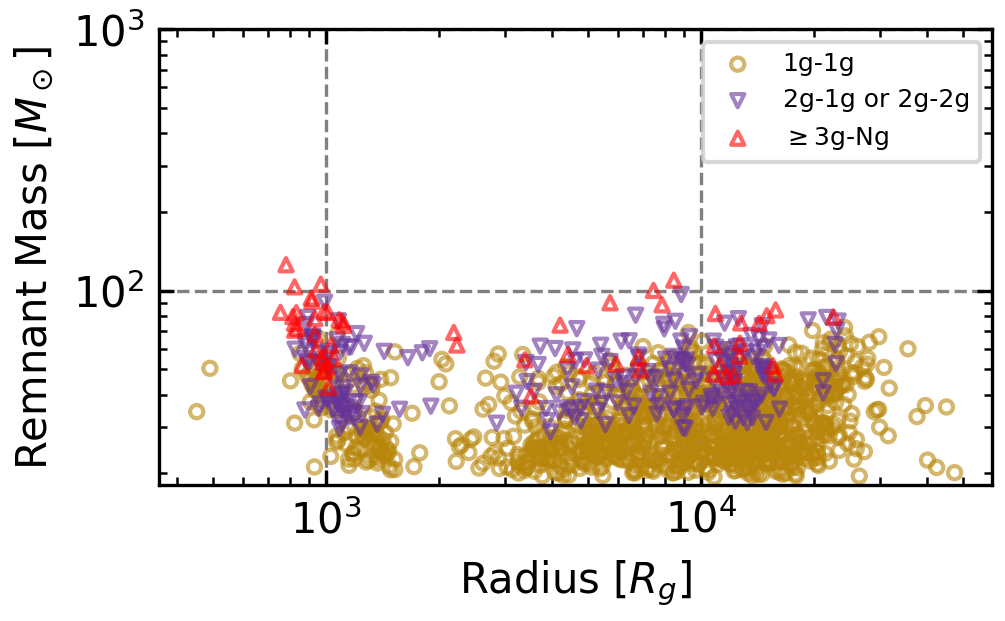
\includegraphics[width=0.5\textwidth]{ch_agnbbh_figs/jm17_m_rad_vf.png}
      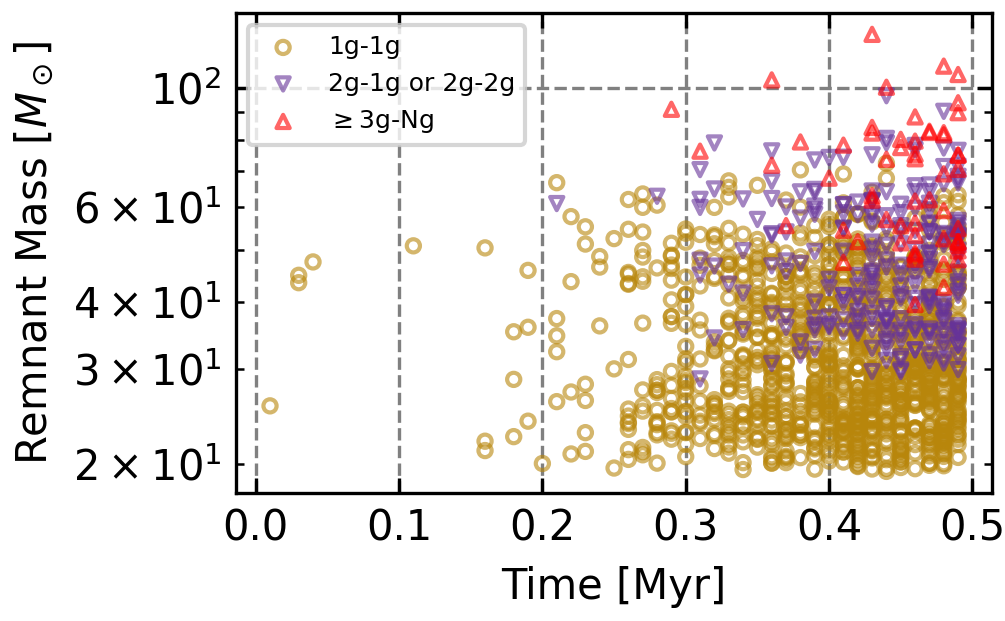
\includegraphics[width=0.5\textwidth]{ch_agnbbh_figs/jm17_time_vf.png}
	\caption[Jimenez \& Masset torque prescription]{\textbf{Jimenez \& Masset torque prescription}As Fig.~\ref{fig:dyn-ecc}, except \texttt{torque\_prescription = jimenez\_masset}. Equivalent merger rate is ${\mathcal{R}} \sim 21.2\ {\rm Gpc}^{-3} {\rm yr}^{-1}$.
   }
    \label{fig:jm}
\end{figure*}


By contrast, Fig.~\ref{fig:ecc} shows what happens if we assume an initially eccentric population (\code{flag_eccentricity_damping = 1} with a uniform eccentricity distribution), with maximum initial eccentricity = 0.9, with otherwise identical input parameters as in Fig.~\ref{fig:circ}. The merger rate drops dramatically to $\mathcal{R}\sim 26.8\, {\rm Gpc}^{-3}{\rm yr}^{-1}$ as a delay time ($\sim 0.03$ Myr) is introduced since it takes time for gas damping to begin building up the circularized BH population. This population will also preferentially occur at thinner regions of the AGN disk, so the migration swamp/trap region remains important but fewer (less massive) IMBH are now produced. 


\subsection{Testing dynamics}
Among a disk BH population where dynamics is ignored, BBHs will tend to form in regions where there is crowding (e.g. near migration traps), as in Fig.~\ref{fig:ecc}. However, things can change once we allow dynamical interactions to occur.

First, we introduce interactions between the embedded BH in the disk. Circularized BH are dynamically heated by close encounters with the eccentric population. This introduces an additional delay time ($\sim 0.3$Myr, excluding a handful of very close initial BH) before BBH can merge in addition to the gas circularization delay time seen in Fig.~\ref{fig:ecc}. The average rate of dynamical encounters among an eccentric BH population is highest in the inner disk and so the circularized population build-up near the migration trap/swamp is inhibited initially, leading to a delay in higher generation mergers. This is clear from Fig.~\ref{fig:dyn-ecc}
 where we assume $e_{\rm max}=0.3$ and the BH populations within the disk (eccentric and circularized) are allowed to interact with each other. Dynamical destruction of inner disk BBH leads to a delay in 3g-ng mergers, which first appear after $\sim 0.4$Myr vs $\sim 0.2$Myr in Fig.\ref{fig:ecc}). As we increase $e_{\rm max}$, the delay-time increases and the AGN needs to run for longer to drive a higher merger rate. Fig.~\ref{fig:jm} shows the effect of choosing a different torque prescription but all else as in Fig.~\ref{fig:dyn-ecc}. The \citet{JimenezMassset17} prescription leads to a lower torque magnitude by $\sim 30\%$ across the outer disk, delaying mergers and inhibiting higher generation mergers for an AGN of the same lifetime (again see Fig.2 of \citep{Grishin+23} for an approximate illustration).

\begin{figure}
    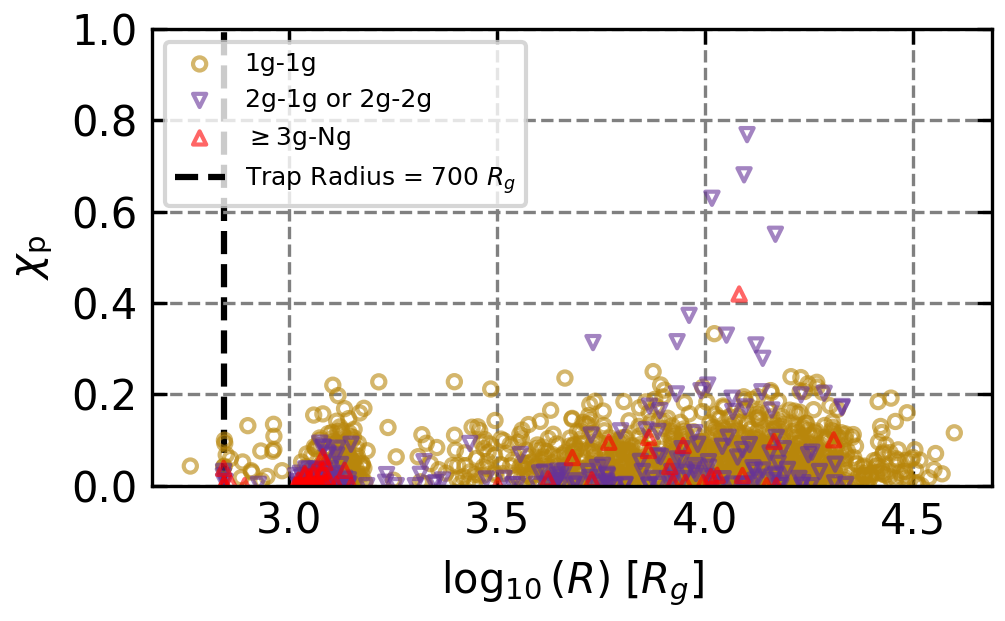
\includegraphics[width=0.5\textwidth]{ch_agnbbh_figs/default_r_chi_p.png}
    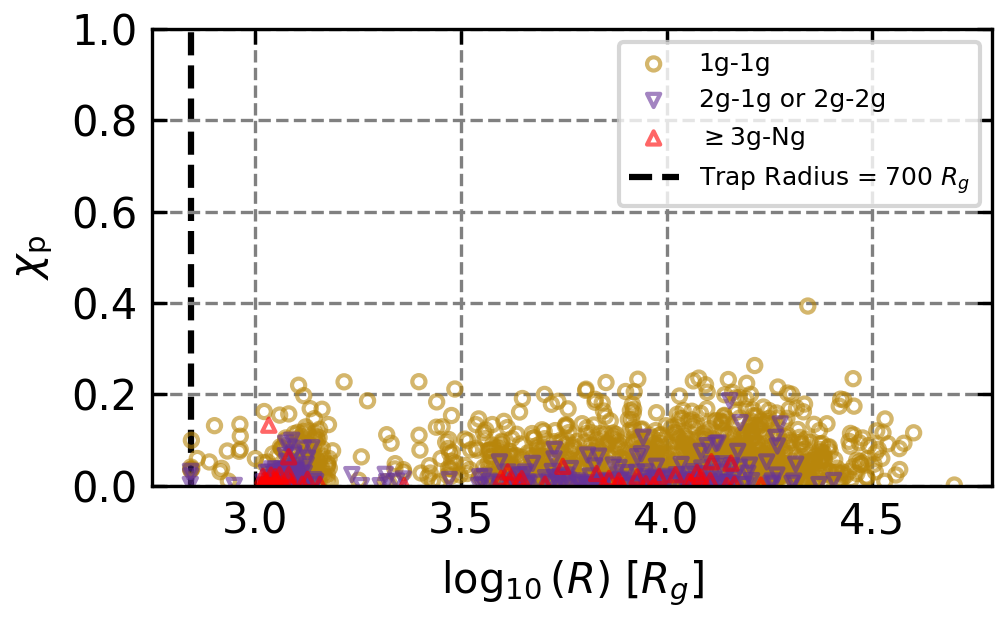
\includegraphics[width=0.5\textwidth]{ch_agnbbh_figs/p123_sphoff_r_chi_p.png}
	\caption[In-plane spin for BBH mergers as a function of disk radius]{\textbf{$\chi_{\rm p}$ for BBH mergers as a function of disk radius} where spheroid encounters are on (top panel) and spheroid encounters are off (bottom panel). Input file and parameters (top panel) are as in Fig.~\ref{fig:dyn-ecc}, and in bottom panel except \texttt{nsc\_spheroid\_normalization = 0.0}. Equivalent merger rate is ${\mathcal{R}} \sim 22.0(22.7) \,{\rm Gpc}^{-3} {\rm yr}^{-1}$ top (bottom) panel.
   }
    \label{fig:chi_p}
\end{figure}


\begin{figure}
    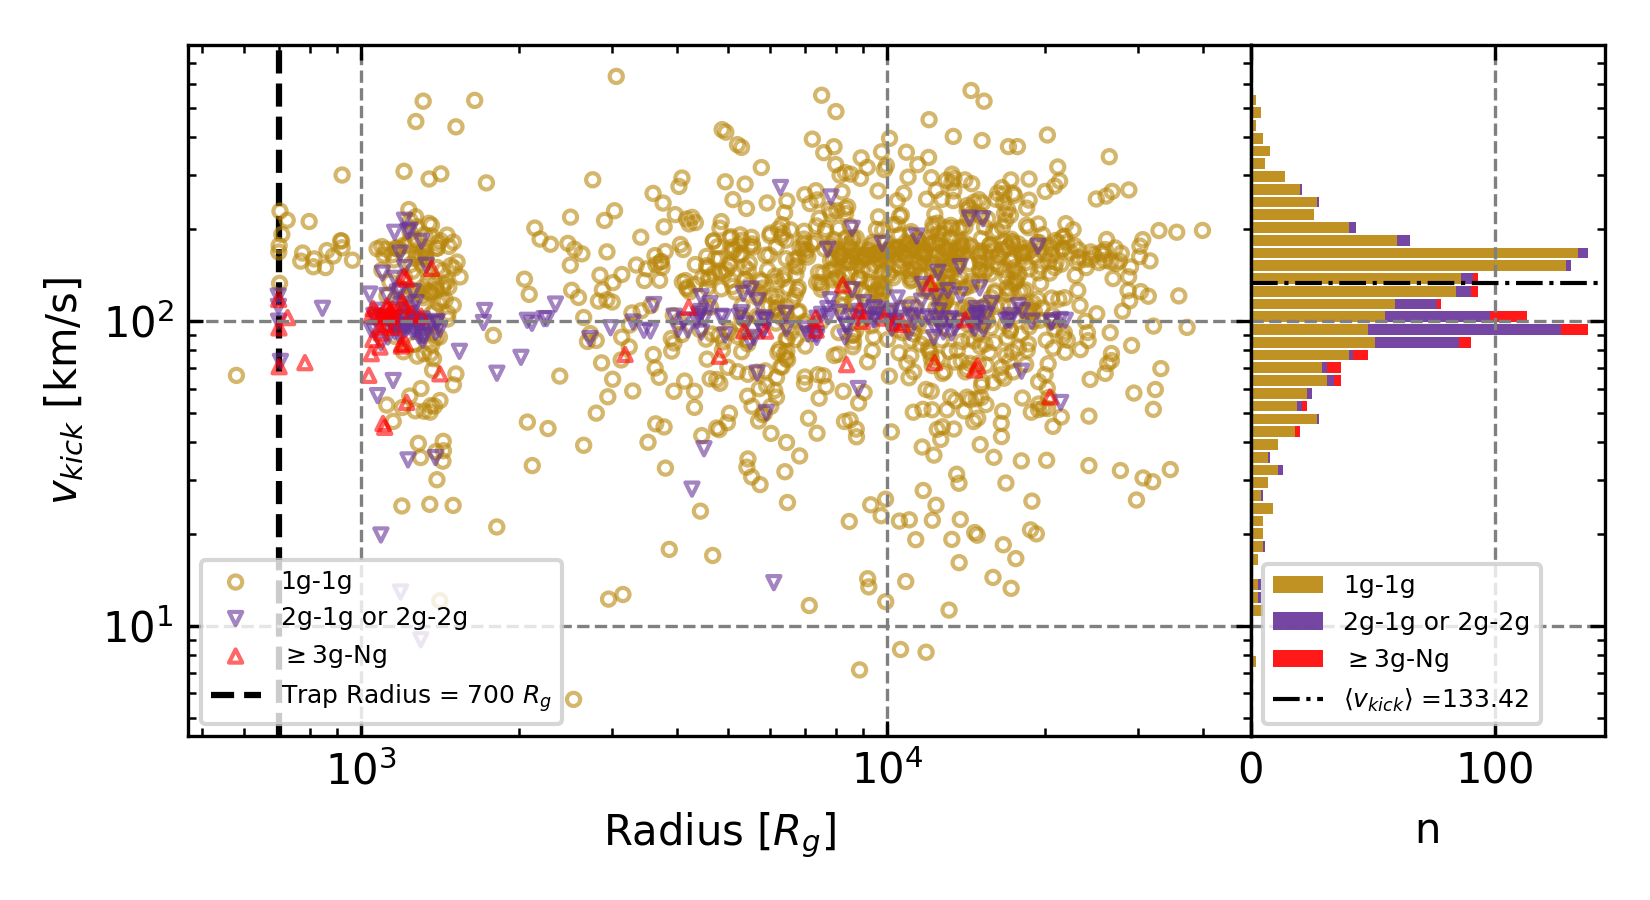
\includegraphics[width=0.5\textwidth]{ch_agnbbh_figs/default_v_kick_vs_radius.png}
	\caption[Velocity kicks vs. radius]{\textbf{Velocity kicks vs. radius.} (\emph{Left panel:})  Velocity kicks as a function of disk radius and generation associated with mergers for the model in Fig.~\ref{fig:mf2}(a). (\emph{Right panel:}) Number and generation of mergers as a function of kick velocity. Dash-dot line corresponds to mean kick velocity of $\sim 133{\rm km/s}$.
    }
    \label{fig:v_kick}
\end{figure}
Dynamically we also introduce encounters between the spheroid NSC population and the embedded BBH population in the disk. Spheroid encounter rates are highest in the inner disk, but with disk dynamics on, the overall effect on the merger rate is small (few $\%$ change). 
Spheroid encounters have a significant effect in generating a in-plane spin component ($\chi_{\rm p}$). Conservation of orbital angular momentum in moderately close interactions between disk BBH and spheroid stars will pop BBH out of the AGN disk with a new orbital angular momentum ($L_{\rm BBH}$) orientation, but individual BH spin alignments do not change, yielding a significant spin component in the plane of $L_{\rm BBH}$ \citep{Tagawa+20spin,Samsing+22,McKernanFord24}. Fig.~\ref{fig:chi_p} shows $\chi_{\rm p}$ as a function of BBH merger location in the disk with spheroid encounters on/off (left/right panel respectively) (\code{nsc_spheroid_normalization=1/0}). The highest values of $\chi_{\rm p}$ are overwhelmingly driven by higher generation (higher mass) mergers. Higher mass BBH have a larger cross-section for spheroid encounters (larger $R_\mathrm{H}$), but higher mass makes them harder to ionize via spheroid stellar encounters. This feature of the AGN channel should be directly testable in O4 by LVK.

Fig.~\ref{fig:v_kick} shows the distribution of merger kick velocities as a function of disk radius, calculated from eqn.~\ref{eq:v_kick}. First generation BH mergers (in gold) peak strongly around $\sim 200{\rm km/s}$ as we expect \citep{Varma+22}. However, higher generation BH have smaller kick magnitudes ($\sim 100{\rm km/s}$) with this prescription. We caution that this is an \emph{underestimate} of the kicks to be expected among higher generation mergers. In particular, including the relativistic evolution of the BBH allows for much higher values of the merger kick (up to $\sim 2000{\rm km/s}$) among the higher generation mergers. This will be very important for potential mass segregation between AGN phases \citep[e.g.][]{Gilbaum+25} (see also Ray et al. 2026, in prep.).

\subsection{The $q$--$\Xeff$ anti-correlation}
\label{sec:qXeff-agnbbh}
LVK observations suggest an intruiging anti-correlation between the BBH mass ratio ($q$) and the effective spin ($\Xeff$) of mergers \citep{Callister21}. The anti-correlation is consistent with greater alignment between spin and BBH orbital angular momentum for the primary BH component ($\chi_{1}$) when BBH masses are less equal. The only reason for such a anti-correlation to arise in a dynamical channel is if there is a bias towards alignment of the primary BH spin with the BBH orbital angular momentum. AGN disks can naturally provide such a bias \citep[e.g.][]{McKernan+22:q-Xeff, Santini+23}. This bias alone (via spin-up and spin torquing) is insufficient however; a bias \emph{against} retrograde BBH mergers is also required. In the AGN channel, such a bias might occur because: (i) Retrograde disk BBH are flipped to prograde over time due to gas accretion \citep{DittmannJermynCantiello23} or, (ii) retrograde BBH experience orbital eccentricity pumping \citep{Calcino+23}, so retrograde BBH should spend more time at wider separations than prograde BBH with similar semi-major axes around their center of mass \citep{WangZhuLin24}, or (iii) spheroid encounters with in-plane retrograde BBH will drive the BBH away from retrograde \citep{Samsing+22} and gas torquing tends to drive the BBH towards $\Xeff>0$. 

\begin{figure*}
    \centering
    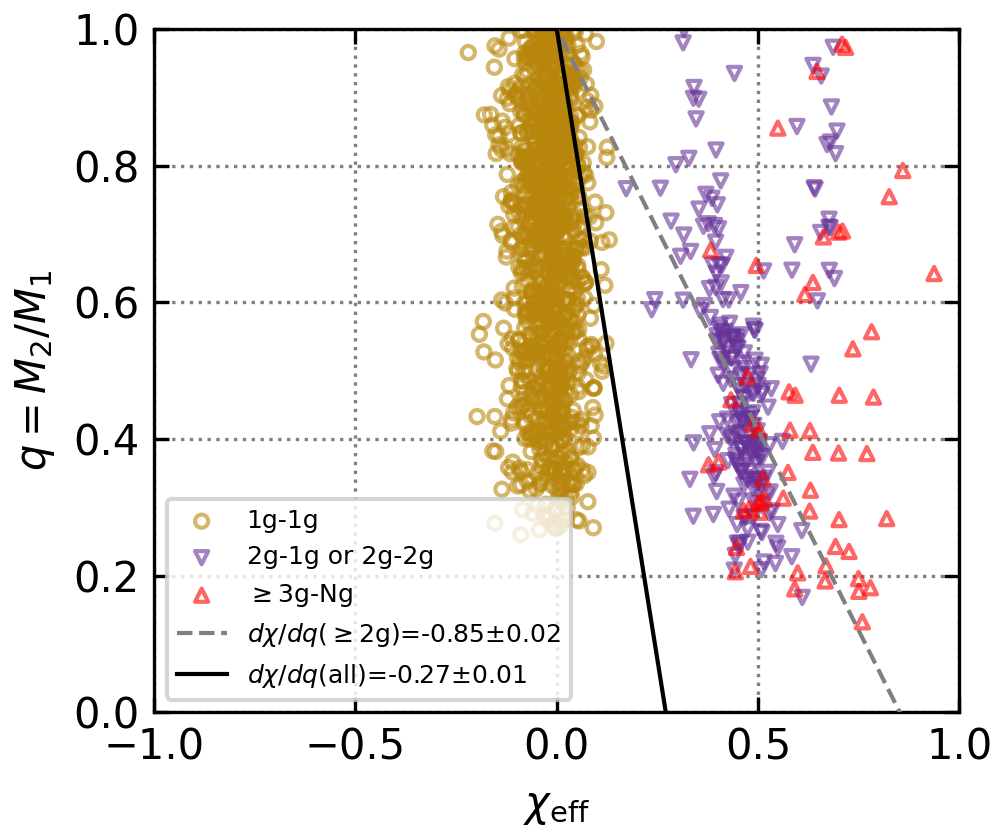
\includegraphics[width=0.5\textwidth]{ch_agnbbh_figs/default_q_chi_eff.png}
    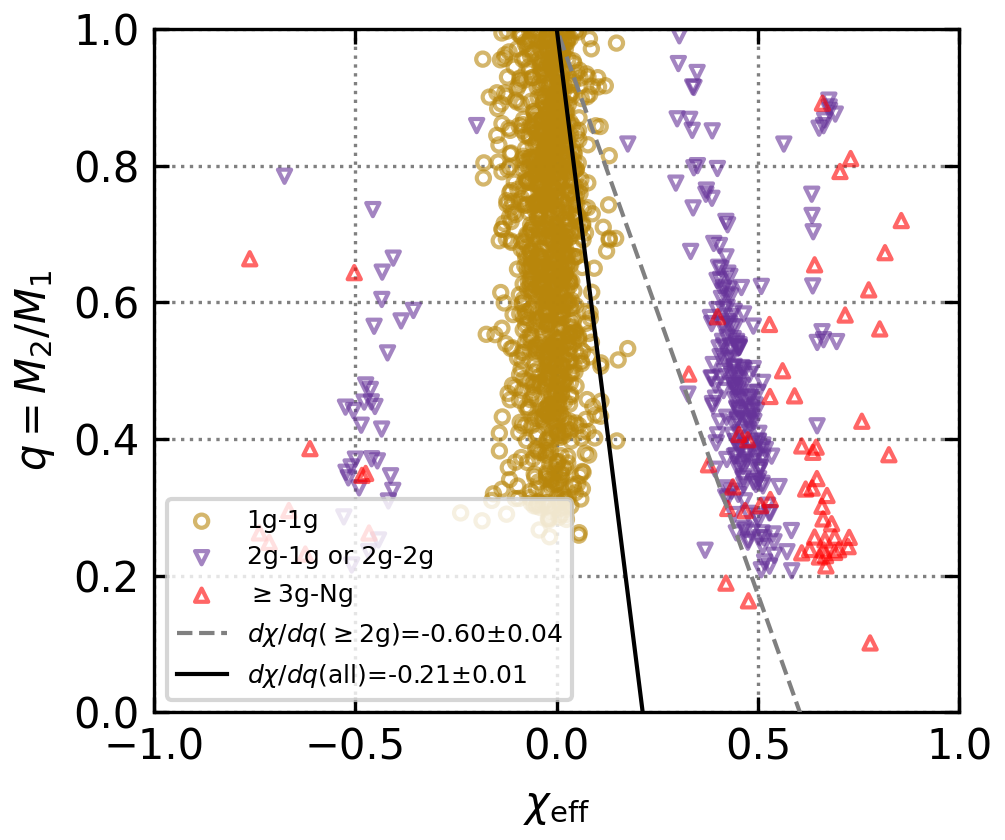
\includegraphics[width=0.5\textwidth]{ch_agnbbh_figs/p123_ret1_q_chi_eff.png}
	\caption[$q$ vs. $\Xeff$]{\textbf{Mass ratio ($q$) distribution as a function of $\Xeff$.} Left panel assumes all BBH are biased to form prograde  and right panel assumes $10\%$ form retrograde. Input file is \texttt{model\_choice\_old.ini} as for Fig.~\ref{fig:dyn-ecc} left panel and in the right panel we assume \texttt{fraction\_bin\_retro=0.1}.  Equivalent merger rates are ${\mathcal{R}} \sim 22.0(22.2) {\rm Gpc}^{-3} {\rm yr}^{-1}.$
   }
    \label{fig:qX}
\end{figure*}

\begin{figure*}
    \centering
    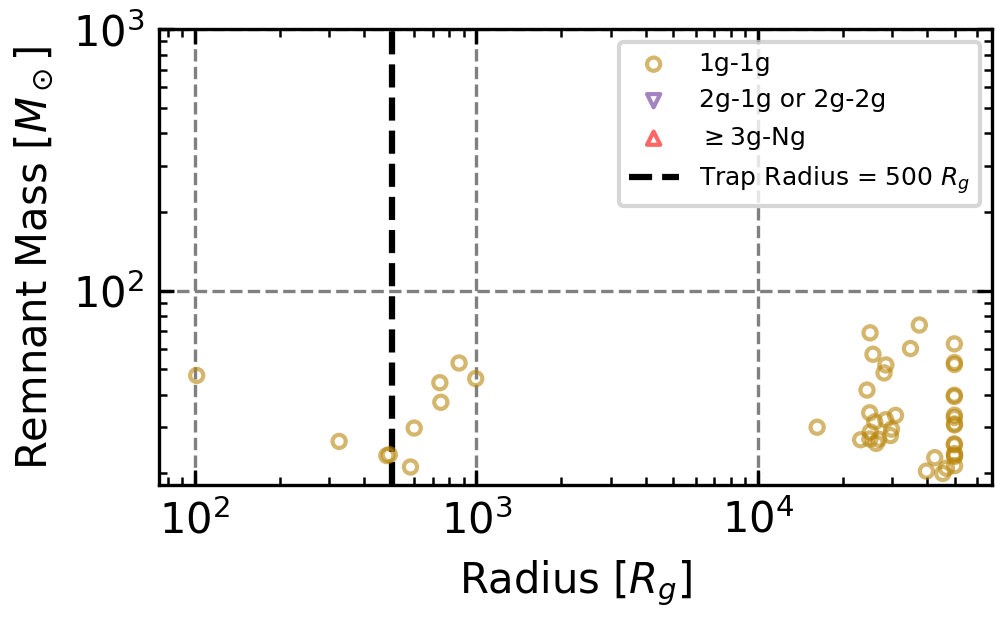
\includegraphics[width=0.5\textwidth]{ch_agnbbh_figs/p123_tqm_merger_mass_v_radius.png}
      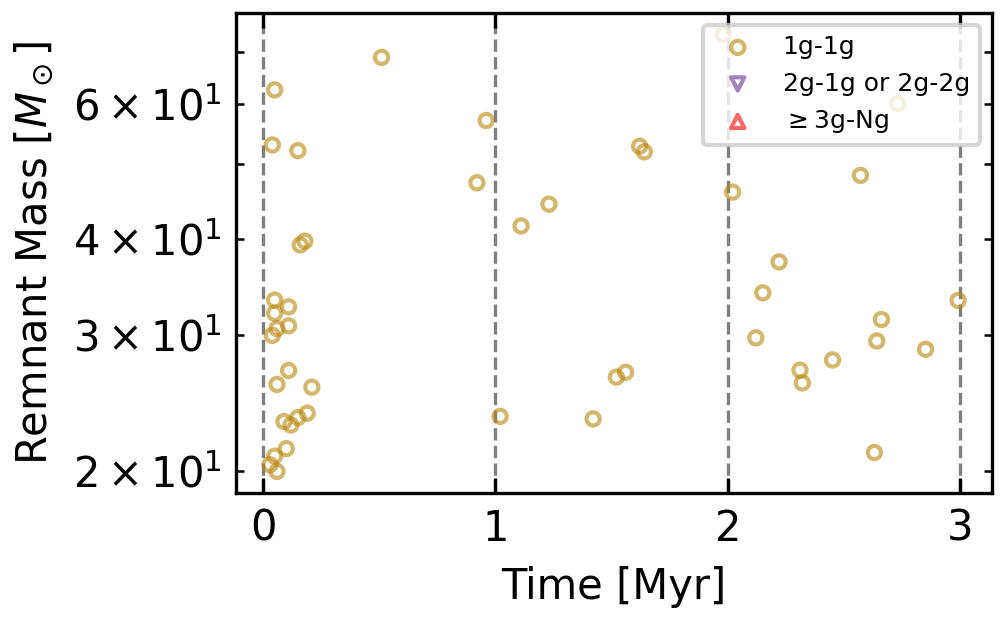
\includegraphics[width=0.5\textwidth]{ch_agnbbh_figs/p123_tqm_time_of_merger.png}
	\caption[Using \code{pAGN} TQM model]{\textbf{Using \code{pAGN} TQM Model.} As Fig.~\ref{fig:dyn-ecc} except uses a \texttt{pAGN} supplied \citet{ThompsonQuataertMurray05} disk model for 3Myr. Input file is as in Fig.~\ref{fig:dyn-ecc} except \texttt{disk\_model\_name = 'thompson\_etal'}. Equivalent merger rate is ${\mathcal{R}} \sim 0.1  {\rm Gpc}^{-3} {\rm yr}^{-1}.$
   }
    \label{fig:tqm_default}
\end{figure*}

\begin{figure*}
    \centering
    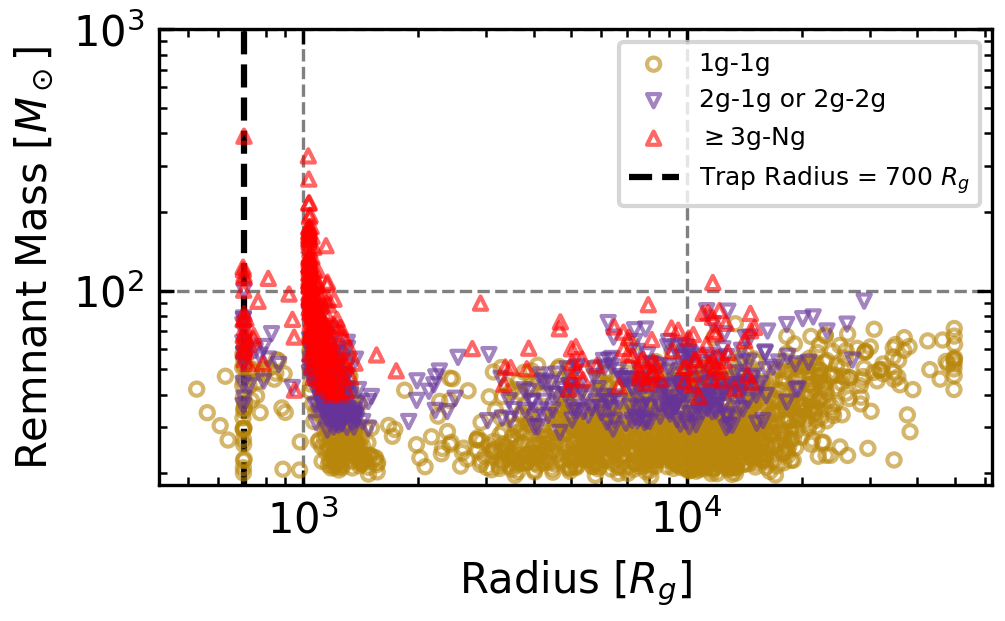
\includegraphics[width=0.5\textwidth]{ch_agnbbh_figs/p123_1Myr_ec9_merger_mass_v_radius.png}
      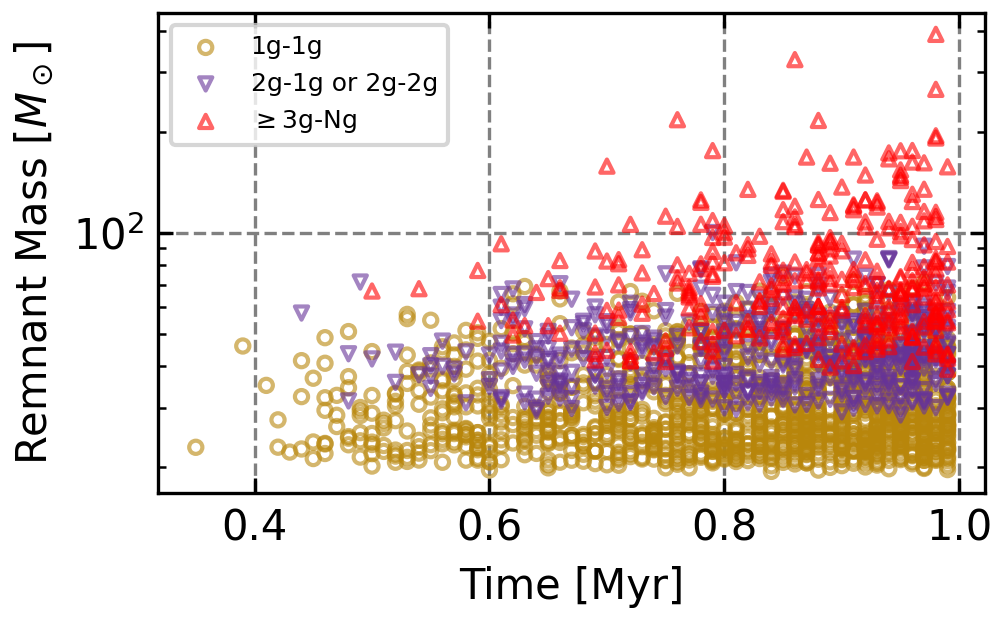
\includegraphics[width=0.5\textwidth]{ch_agnbbh_figs/p123_1Myr_ec9_time_of_merger.png}
	\caption[Disk lifetime of 1 Myr]{\textbf{Disk lifetime of 1 Myr.} As Fig.~\ref{fig:dyn-ecc} except disk runs for 1Myr. Input file and parameters are as in Fig.~\ref{fig:dyn-ecc} except \texttt{timestep\_num = 100}. Equivalent merger rate is ${\mathcal{R}} \sim 41.2 {\rm Gpc}^{-3} {\rm yr}^{-1}.$
   }
    \label{fig:sg_dyn_on_5Myr_time}
\end{figure*}


Fig.~\ref{fig:qX} illustrates the $q$--$\Xeff$ distribution for our default model, assuming the retrograde:prograde fraction of BBH mergers is $0(0.1)$ in the left(right) panel. Most mergers are 1g-1g and center around $\Xeff=0$. Higher generation mergers ($ng-mg$) ($n\geq 2,m \geq 1$) are mostly displaced to $|\Xeff| \sim [0.3,0.7]$ with more massive primaries typically having a spin that dominates the $\Xeff$ calculation. The width of the 1g-1g distribution depends on the choice of initial BH spin magnitude distribution and the extent of the 1g-1g distribution in $q$ is a function of the BH IMF ($M_{\rm BH,min/max}$). Thus, the $q$--$\Xeff$ distribution is an effective test of the BH IMF and spin distribution in galactic nuclei.
A full parameter space study can be found in \citep{Cook+25}.


\subsection{Testing AGN disk models}
\label{sec:disks}
We picked two AGN disk models to test, namely \citet{SirkoGoodman03} and \citet{ThompsonQuataertMurray05}.
Our default model is \citet{SirkoGoodman03} since this tends to give a better fit to the UV `big blue bump' in quasar spectral energy distributions and we expect that dense quasar disks are more efficient at coagulating embedded populations. In the case of \citet[][hereafter TQM]{ThompsonQuataertMurray05}, this disk model is less dense, less optically thick and at least nominally allowed to have a migration trap at $500\Rg$ \citep{Bellovary+16}, although this is likely due to an incorrect modelling of opacities \citep{DittmannMiller20}.

For reference, \Fig{fig:sg-disk} from the \citet{SirkoGoodman03} shows their disk radial profiles for an SMBH mass $\Mbh=10^8\,\Msun$ and Eddington ratio $l_\text{E}=L_0/L_\text{E}=0.5$ where the Eddington luminosity $L_\text{E} = \epsilon\dot{M}c^2$ for a non-self-gravitating disk with mass accretion rate $\dot{M}$ and $\epsilon=0.1$.
In comparison, \Fig{fig:tqm-disk} from \citet{ThompsonQuataertMurray05} shows their disk radial profiles for $\Mbh=10^9\,\Msun$, the mass accretion rate feeding the outer edge of the disk $\dot{M}_\text{out}=320\,\Msun\ \text{yr}^{-1}$ at $R_\text{out}=200$ pc, and a mach number $\text{Ma}=v/\cs=0.2$.

\begin{figure}
\centering
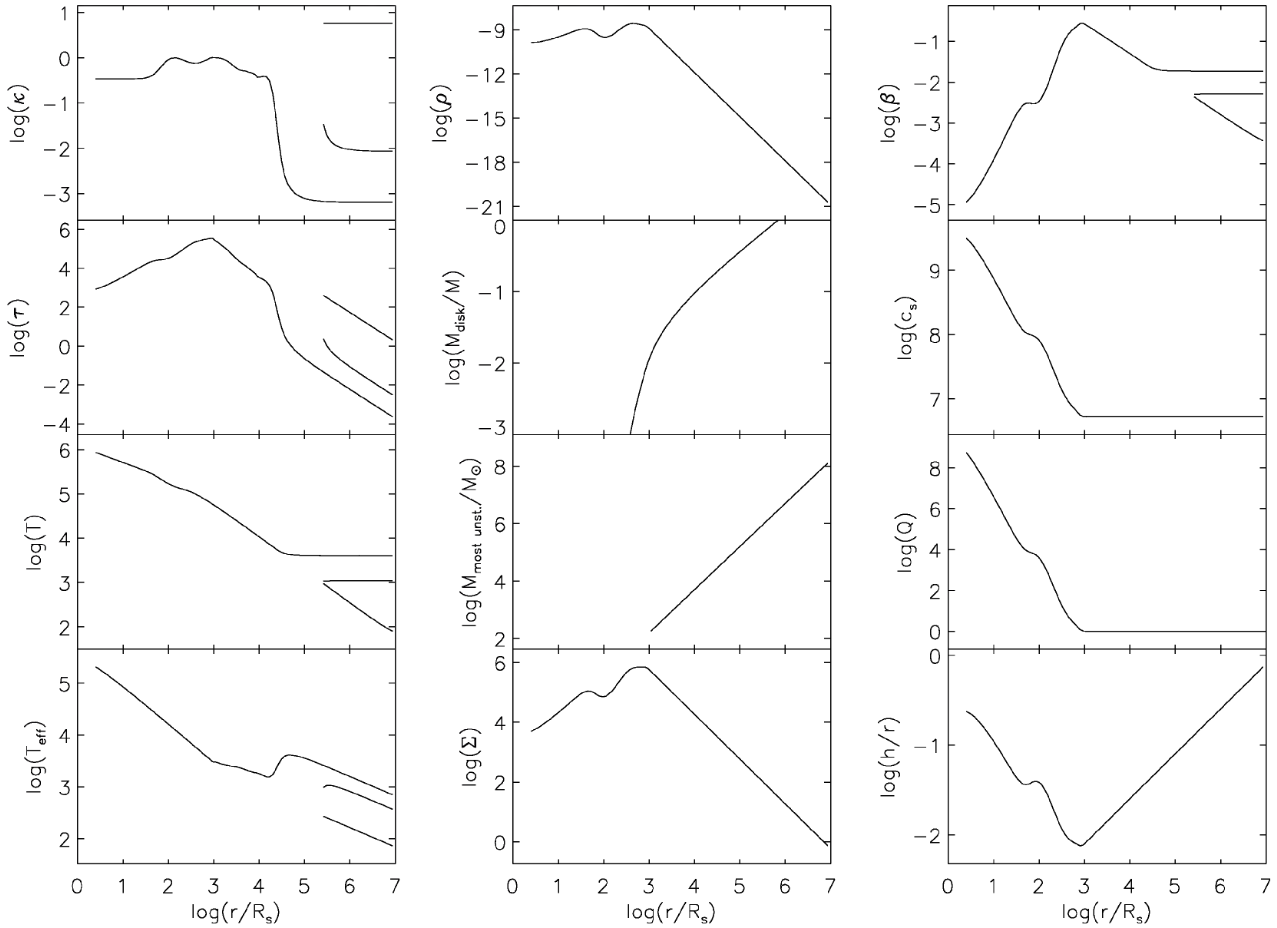
\includegraphics[width=1\textwidth]{ch_agnbbh_figs/sg_disk.png}
	\caption[Sirko and Goodman disk model]{\textbf{Sirko and Goodman disk model.} Radial AGN disk profiles for $\Mbh=10^8\,\Msun$ and $l_\text{E}=0.5$.
Reproduced from \citet{SirkoGoodman03}.}
\label{fig:sg-disk}
\end{figure}

\begin{figure}
\centering
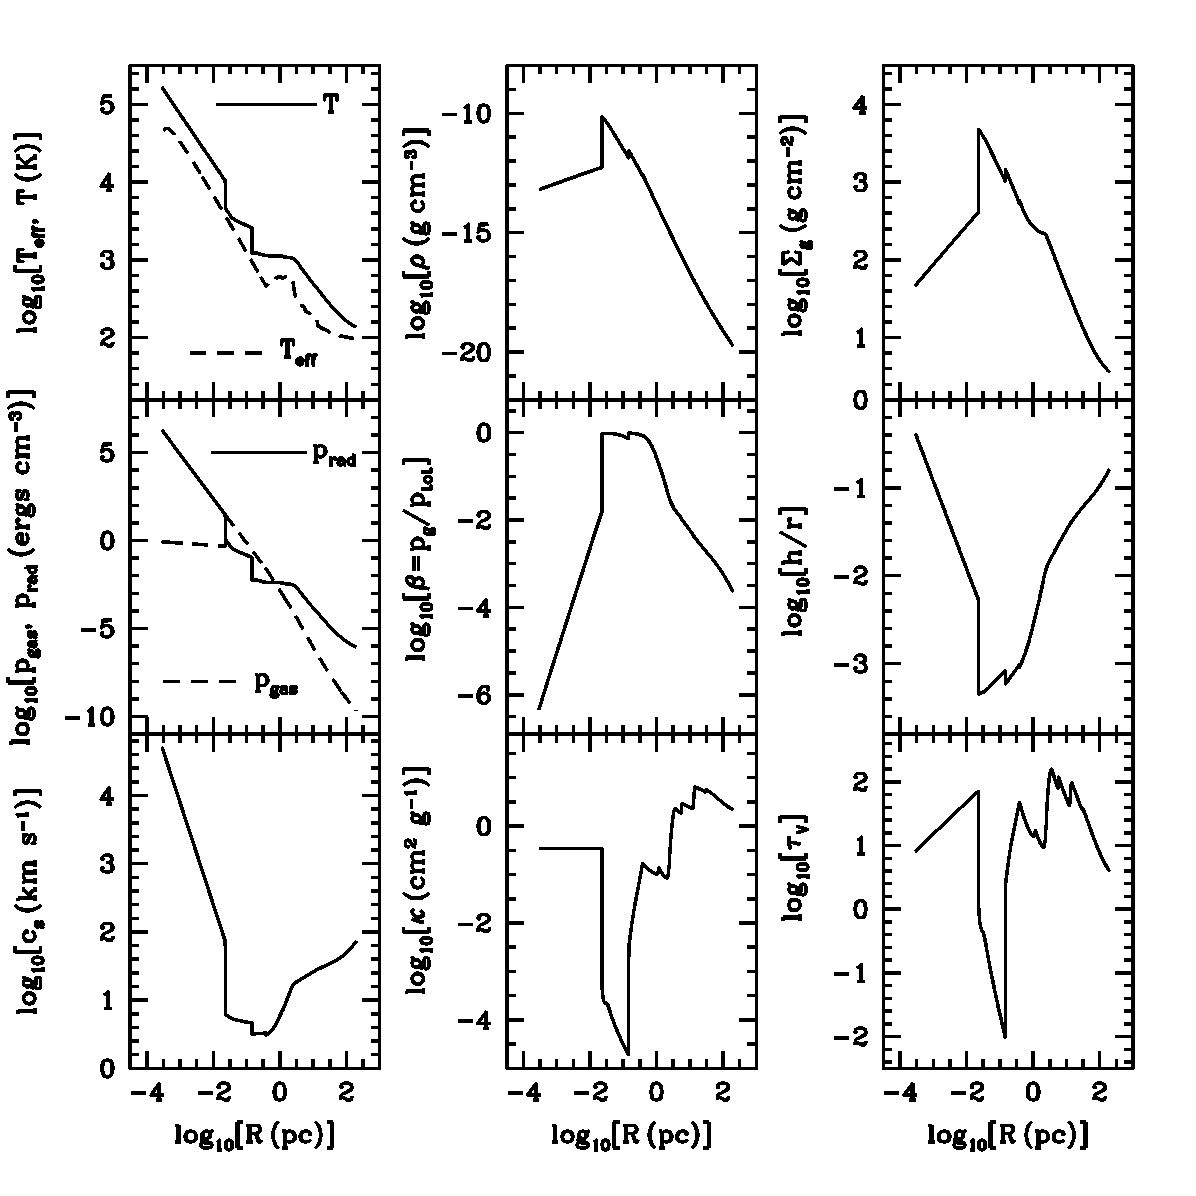
\includegraphics[width=1\textwidth]{ch_agnbbh_figs/tqm_disk.pdf}
	\caption[Thompson, Quataert \& Murray disk model]{\textbf{Thompson, Quataert \& Murray disk model.} Radial AGN disk profiles for $\Mbh=10^9\,\Msun$, $\dot{M}_\text{out}=320\,\Msun\,\text{yr}^{-1}$, $R_\text{out}=200$ pc, and $\text{Ma}=0.2$.
Reproduced from \citet{ThompsonQuataertMurray05}.}
\label{fig:tqm-disk}
\end{figure}


Fig.~\ref{fig:tqm_default} shows the distribution of BBH masses as a function of disk radius (left panel) and merger time (right panel) for our default \citet{ThompsonQuataertMurray05} model. Evidently, a less dense disk drives a significantly lower average merger rate ($\sim 0.1 \,{\rm Gpc}^{-3}{\rm yr}^{-1}$) than the \citet{SirkoGoodman03} model and the formation of new BBH becomes more difficult. The LVK AGN channel is likely filled with contributions from both high and low density disks.  Thus, in future work, we will introduce a prior spheroid binary fraction, which could be hardened towards merger, even in very low density AGN disks and which might dominate their contribution to the observed rate.

\subsection{Towards constraints on AGN lifetime}
\label{sec:time}
Fig.~\ref{fig:sg_dyn_on_5Myr_time} shows BBH merger masses as a function of location in disk and time for our default model run for 1Myr with $\rm{e}_{\rm max}=0.9$. The patterns observed in the shorter lived disk model Fig.~\ref{fig:dyn-ecc} persist (left panel) and mergers are delayed by $\sim 0.4{\rm Myr}$ by damping from a higher average initial eccentricity (right panel). The average equivalent merger rate is $\mathcal{R} \sim 41.2\,{\rm Gpc^{-3} yr^{-1}}$. As we limit the AGN fraction of LVK mergers, we will gain strong constraints on the average $\tau_{\rm AGN}$ and we will explore this in future work.


\subsection{Testing GW multi-wavelength models}
\label{sec:gw}
BBH that merge in AGN will be detectable across multiple GW frequencies ($\nu_{\rm GW}$) given by
\begin{equation}
    \nu_{\rm GW} = \frac{G^{1/2}M_{\rm BBH}^{1/2}}{\pi a_{\rm BBH}^{3/2}}
\end{equation}
where $G$ is the universal gravitational constant, $M_{\rm BBH}$ is the BBH total mass and $a_{\rm BBH}$ is the semi-major axis of the BBH around its own center of mass. The resulting gravitational wave strain is
\begin{equation}
    h = \sqrt{\frac{32}{5}} \frac{G^{2}}{c^{4}}\frac{M_{\rm BBH}\mu_{\rm BBH}}{D a_{\rm BBH}}
\end{equation}
with $c$ the speed of light, $\mu_{\rm BBH}=M_{1}M_{2}/M_{\rm BBH}$ is the BBH reduced mass, where $M_{1,2}$ are the masses of the individual BBH components and $D$ is the distance to the BBH. Importantly, in AGN, binary black holes (BBH) can form between two stellar mass BH, but also between individual stellar mass BH and the central SMBH. The latter (SMBH-BH binaries) will be detectable at low GW frequencies as extreme mass ratio inspirals (EMRIs) with LISA \citep{LISA23}.

As BBH evolve (due to gas hardening/softening, binary softening/hardening or GW emission) they change their GW frequency. A useful parameter, the characteristic strain, averaged over all polarizations is
given by $h_{\rm char} = (N/8)h$ where $N = \sqrt{2\nu_{\rm GW}^{2}/\dot{\nu}_{\rm GW}}$ and $\dot{\nu}_{\rm GW}=\mathcal{M}_{\rm ch}^{5/3}\nu_{\rm GW}^{11/3}$ where the binary chirp mass $\mathcal{M}_{\rm ch}=(M_{1}M_{2})^{3/5}/M_{\rm BBH}^{1/5}$ if $\nu_{\rm GW}>10^{-6}\,{\rm Hz}$. 

Fig.~\ref{fig:gw_strain} shows the characteristic strain  ($h_{\rm char}$) as a function of gravitational wave frequency ($\nu_{\rm GW}$) assuming all AGN are located at $z=0.1$ by default. For detailed simulations and predictions of redshift dependency of the outputs produced by \code{McFACTS} as a function of $M_{\rm SMBH}$ and NSC properties see \citet{Delfavero+25-mcfactsIII}. Curves in blue (orange) correspond to the LISA (LIGO Hanford O3) sensitivity curves respectively. Note that the LIGO curve is appropriate for $h_{0}$ rather than $h_{\rm char}$. Points in blue correspond to snapshots at the end of each default timestep of EMRIs from 100 iterations of the default model (see Ford et al. 2026 in prep.). Points in gold, purple, red correspond to snapshots of 1g,2g and $\geq 3$g BBH at the end of each timestep of individual BBH with $\nu_{\rm GW}>10^{-7}\,{\rm Hz}$. 

On average $2-3$ points are associated with each BBH, since our default gas hardening prescription \citep{Baruteau11} drives rapid mergers of hard binaries. Once a BBH shrinks to a point where it will merge within the next timestep ($\mathcal{O}(10^{-3}{\rm Hz})$ for default), $\dot{\nu}_{\rm GW}$ in $N$ above is switched from gas-hardening to GW hardening \citep{Peters64}, leading to the break in $h_{\rm char}$ around $\sim 10^{-3}{\rm Hz}$  The first BBH point is arrival in the LISA frequency band on a single timestep, a second BBH point is the evolved BBH in the next timestep, which could correspond to a merger in the LIGO band, or a dynamically hardened/softened BBH (see Postiglione et al. 2026 for a detailed study, and for an illustration of the range of possible BBH merger tracks). BBH that enter the LISA band, but are then ionized, are typically represented by a single point on this plot.  The band of gold, red and purple points correspond to snapshots of BBH mostly gas-hardening towards merger with typical value of $h_{\rm char} \approx \mathcal{O}(10^{-22})$. 
Since binary hardening or softening in the code is either gas-driven or dynamics driven, we have not yet combined gas and dynamics hardening in a given timestep. More sophisticated treatment of both gas and dynamical hardening will be treated in future work ({Postiglione et al. 2026 in prep.}), particularly with a view to testing LISA detectability of gas and dynamically hardened AGN channel BBH. 

\begin{figure}   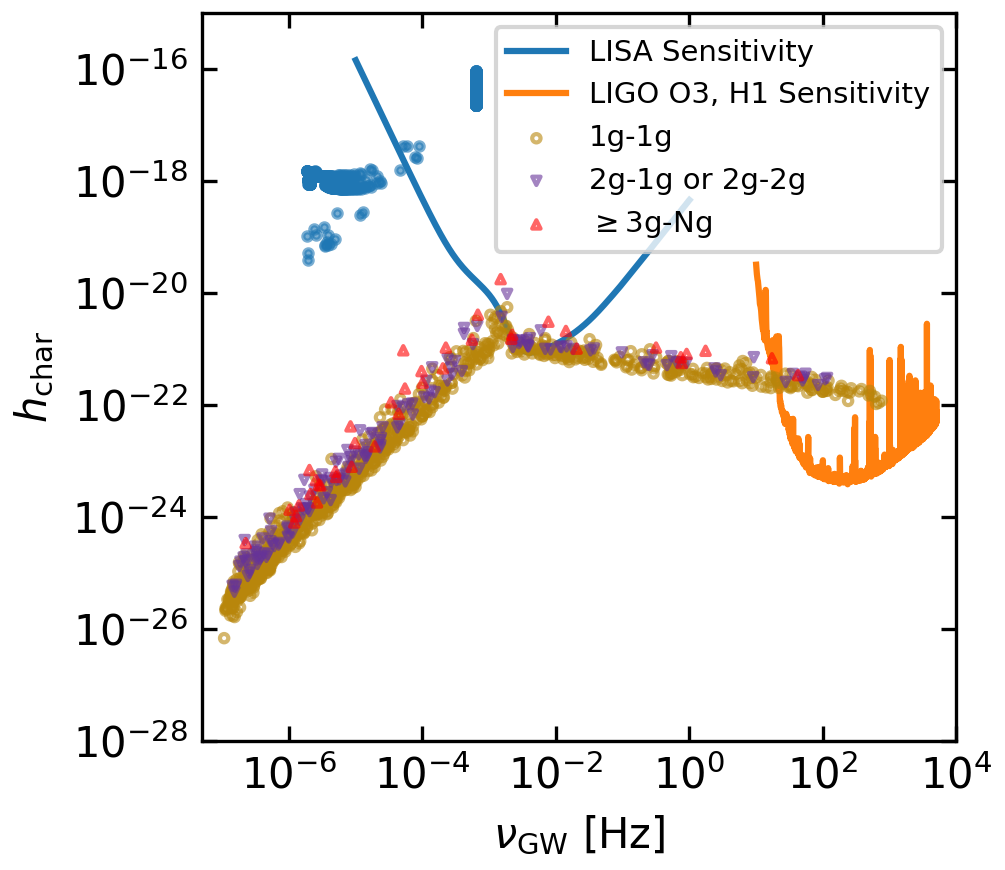
\includegraphics[width=1\textwidth]{ch_agnbbh_figs/gw_strain.png}
	\caption[Characteristic strain vs. frequency]{\textbf{Characteristic strain ($h_{\rm char}$) as a function of GW frequency ($\nu_{\rm GW}$)} after a 0.5Myr episode with default AGN model assumed to lie at $z=0.1$. Note that the LVK sensitivity curve is appropriate for $h_{0}$ rather than $h_{\rm char}$ (see Postiglione et al. 2026 in prep. for a more accurate treatment). Input file and parameters are as in Fig.~\ref{fig:dyn-ecc}.
    }
    \label{fig:gw_strain}
\end{figure}

In \code{McFACTS}, EMRIs form when a BH arrives within $a<50\,\Rg(M_{\rm SMBH}/10^{8}\,M_{\odot})^{-1}$ of the SMBH. The rate at which BH appear at such small disk radii is strongly effected by two factors: first, the number of retrograde embedded BH initially in the disk and second, the rate of disk capture and the range of allowed capture radii. 

When an AGN disk arrives in a relaxed galactic nucleus population, around half of the initial population of orbiters embedded in the disk will have orbits that are retrograde with respect to the disk gas. Depending on their semi-major axis and the disk surface density profile, the gas can excite the orbital eccentricity of embedded retrograde BH to large values, potentially generating a population of BH at small disk radii \citep{Secunda+21}. However, perturbations of orbital inclination of embedded retrograde orbiters, due to e.g. turbulence, or interactions with spheroid orbiters, will tend to drive the retrograde orbiters out of the disk and tend to rapidly flip them to prograde \citep{WangZhuLin24}. This initially retrograde population in a turning-on AGN will tend to drive a high EMRI rate (these correspond to the vertical line of blue points at $\nu_{\rm GW} \sim 10^{-3}{\rm Hz}$ in Fig.~\ref{fig:gw_strain} and see {Ford et al. 2026 in prep.}). After multiple short-lived AGN episodes in the same nucleus, the retrograde fraction in the disk should become very small, so the LISA EMRI rate should be highest in new AGN episodes in relatively relaxed galactic nuclei (Ford et al. 2026 in prep.).

Under default models, the disk captures BH uniformly at radii $a<2\times 10^{3}\,\Rg$ every 0.1Myr, so there is a $2.5\%$ chance of an EMRI every disk capture under default assumptions. EMRIs are considered to only evolve under the evolution of GW emission (gas effects are ignored for now). So in Fig.~\ref{fig:gw_strain} the characteristic strain per frequency (equivalently the amount of time at a monochromatic 
 GW frequency) decreases as the EMRI shrinks (as $\nu_{\rm GW}$ increases). The exception occurs during the chirp at merger where $h$ increases dramatically. Some EMRIs form late in a run or at large enough distance ($\sim 50\,\Rg$) and do not chirp within the 0.5Myr lifetime. These correspond to the population at lower characteristic strain ($h_{\rm char}/\nu_{\rm GW} \sim 10^{-19}$ in Fig.~\ref{fig:gw_strain}).
 
\subsection{Conclusions}
\label{sec:mcfacts-conclusions}

We demonstrate the new, public, open source, fast and reproducible code $\code{McFACTS}$ , the Monte Carlo For AGN channel Testing and Simulation. \code{McFACTS} allows rapid testing of BBH merger properties across AGN and NSC parameter space. Users can choose their own AGN disk model or NSC model and quickly get population statistics and distributions of parameters. The code as released (\code{v.0.3.0}) makes multiple simplifying assumptions but is intended to be a living, developing code (see \sect{sec:chapter-future} for planned near-future additions).

We illustrate the code and demonstrate its performance by varying AGN and NSC parameter inputs and show that a high average rate ($\mathcal{R}$) of BBH mergers in the AGN channel is generally associated with relatively dynamically cool populations of BBH in short-lived AGN.
This may imply a strong contribution to the LVK AGN channel from AGN fuelled by pulses of low angular momentum gas in the same plane from a fuel reservoir.
For a study of mergers in AGN as a function of NSC model, Galaxy mass and redshift, see \citet{Delfavero+25-mcfactsIII}.
The next chapter will present a detailed studies of the AGN channel in $q$--$\Xeff$ parameter space published in \citet{Cook+25}.

